%%
%% (
%%  )\ )                             (
%%  (()/(   (            (             )\  )   (
%%   /(_))  ))\   (       ))\  (   (   (()/(   ))\
%%   (_))  /((_)  )\  )  /((_) )\  )\   ((_))/((_)
%%   | _ \(_))(  _(_/( (_) )  ((_)((_)  _| |(_))
%%   |   /| || || ' \))/ -_)/ _|/ _ \/ _` |/ -_)
%%   |_|_\ \_,_||_||_| \___|\__|\___/\__,_|\___|
%%

\documentclass{article}
\usepackage[utf8x]{inputenc}
\usepackage{amsmath}
%\usepackage{slashbox}
\usepackage{amsfonts}
\usepackage{amssymb}
\usepackage{graphicx} % Paquete para incluir imágenes en el documento LaTeX
\usepackage{hyperref}
\hypersetup{
  colorlinks=true,
  linkcolor=blue,
  filecolor=magenta,
  urlcolor=cyan,
}
\urlstyle{same}
\usepackage{varwidth}

\newcommand\tab[1][1cm]{\hspace*{#1}}

\usepackage{multirow}

\usepackage[a4paper,rmargin=1.5cm,lmargin=1.5cm,top=1.5cm,bottom=1.5cm]{geometry}

\usepackage{pdfpages}

\usepackage{xcolor}
\usepackage{minted}
\setminted[mysql]{frame=lines, framesep=2mm, baselinestretch=1.2, rulecolor=\color{black!80}, bgcolor=DarkGray}
\usemintedstyle[mysql]{monokai}
\setminted[python3]{frame=lines, framesep=2mm, baselinestretch=1.2, rulecolor=\color{black!80}, bgcolor=DarkGray}
\usemintedstyle[python]{paraiso-dark}
\setminted[./pseudocode.py:PseudocodeLexer -x]{frame=lines, framesep=2mm, baselinestretch=1.2,
            rulecolor=\color{black!30}, bgcolor=LightGray}
\usemintedstyle[./pseudocode.py:PseudocodeLexer -x]{rainbow_dash}
\setminted[bash]{baselinestretch=1.2,rulecolor=\color{black!30},fontsize=\footnotesize,bgcolor=LightGray}
\definecolor{LightGray}{gray}{0.98}
\definecolor{DarkGray}{gray}{0.1}
\definecolor{MidGray}{gray}{0.8}
\definecolor{codegreen}{rgb}{0,0.6,0}
\definecolor{codegray}{rgb}{0.5,0.5,0.5}
\definecolor{codepurple}{rgb}{0.58,0,0.82}
\definecolor{backcolour}{rgb}{0.95,0.95,0.92}

\setlength{\parindent}{0px}  % Setea la indentacion de la primera linea de cada parrafo a cero pixeles.


\title{Resolución de la novena semana}
\author{@RuneCode}

\begin{document}
%% Portada
\includepdf{./portada/portada.pdf}

\section{Bienvenida conceptos básicos y contexto histórico de las Bases de Datos}%

\textbf{Historia de Base de datos}

Desde la antiguedad se quería tener persistencia de la información y para esto
se desarrollaron sistemas de escritura en piedra o arcilla, luego el papiro que
permitía mayor portabilidad de los documentos pero no eran tan resistentes ya
que se descomponían o eran anidados por hongos y finalmente los chinos que
inventaron el papel que tenía las ventajas de ser fáciles de transportar pero
también muy resistentes.

Pasaron muchos siglos y el siguiente salto que se logró después del papel se
dio en el siglo XX con el microfilm que tiene la ventaja de almacenar
información que puede durar miles de años sin ningún problema, la desventaja es
que el guardar información, modificar y leer información requiere máquinas muy
especializadas que no son fáciles de conseguir y no es tan fácil el proceso.

Luego tenemos a los medios digitales: Los discos duros, discos de estado
sólido, incluso los CDs fueron medios de almacenamiento digital en los que para
su almacenamiento se usó el formato digital de "unos y ceros".

El siguiente gran cambio que se dió fue la nube. La nube tiene como beneficio a
su favor el que es accesible desde cualquier parte del mundo.

Entonces ¿Qué son las Bases de Datos?
Las bases de datos entran en el periodo en el que hicimos la transición a
medios digitales y ahora en la nube.
Las bases de datos nos servian para complementar la arquitectura de Von Neumann
(que es la arquitectura de computación clásica que contiene un CPU, memoria y
elementos de entrada y salida).

Las bases de datos se han divido en dos grandes tipos, las Relacionales, que
fueron las primeras en surgir y luego las no relacionales.

Con respecto a las Base de Datos relacionales actualmente tenemos en la
industria varias compañías que se dedican a ser manejadores de Base de Datos
Relacionales, por ejemplo SQL Server de Microsoft, luego Oracle que ha sido muy
popular e importante; pero tenemos también las versiones de comunidad u Open
Source, por ejemplo PostgresSQl, la más usada probablemente en la industria que
es MySQL que aunque ahora pertenece a Oracle anteriormente era de Sun
Microsistem y como respuesta a esta adquisición de MySQL también se crea
MariaDB que es virtualmente lo mismo que MySQL de hecho es un fork del codigo
original que hizo su creador para continuar con este proyecto de una manera más
libre sin tener que estar atado a Oracle.

Con respecto a la Base de Datos no Relacionales es un mundo muy interesante y
que todavía está avanzando por ejemplo: MemcacheDB, Cassandra que es una base
datos que inventó Facebook, DynamoDB, elasticsearch, BigQuery, y también
tenemos algunas muy interesantes como: neo4j (basada en grafos), MongoDB (una
de las más utilizadas) y tenemos firestore que es una muy reciente.

Tenemos también otra gran división de servicios de Base de Datos: Los que se
llaman Autoadministrados y los Administrados. Los Autoadministrados, es la base
de datos que tu instalas en tu computadora o en tu servidor, tu te encargas de
las actualizaciones y te encargas de toda la parte de mantenimiento,
actualización, parche, persistencia de datos, etc. Los servicios administrados
por otro lado no los llevar tu, son servicios que ofrecen las nubes modernas,
por ejemplo: Amazon, Google o Azure de Microsoft que lo que te ofrecen es
realmente el servicio de base de datos. Tu vas a usarla pero no tienes que
instalarla u ocuparte de todo el mantenimiento que implica. Como se ve ambas
tienen ciertas ventajas y desventajas.

%% clase 2
\section{Historio de las RDB}%
Las bases de datos surgen de la necesidad de conservar la información más allá
de lo que existe en la memoria RAM. Y cuando tuvimos la necesidad de guardar la
información de una forma que fuera facil de guardar y extraer empezaron a
buscarse formas un poquito más inteligentes de hacerse esto. La primera
aproximación fueron lo que se llaman Base de Datos basados en archivos que no
es lo mismo que Base de Datos basados en Documentos.

Las bases de datos surgen de la necesidad de conservar la información mas allá
de lo que existe en la memoria RAM en el esquema de la arquitectura de Von
Neumann.

Las bases de datos basadas en archivos eran datos guardados en texto plano,
fáciles de guardar pero muy difíciles de consultar y por la necesidad de
mejorar nacen las \textbf{bases de datos relacionales}. Su inventor
\textbf{Edgar Codd} dejó ciertas reglas para asegurarse de que toda la
filosofía de las bases de datos no se perdieran, estandarizando el proceso.\\

Codd inventó algo llamado el Álgebra Relacional.

%% Clase 3
\section{Entidades y atributos}%
Una \textbf{entidad} es algo similar a un objeto (programación orientada a
objetos) y representa algo en el mundo real, incluso algo abstracto. Tienen
atributos que son las cosas que los hacen ser una entidad y por convención se
ponen en plural.

\begin{figure}[h!]
    \centering
      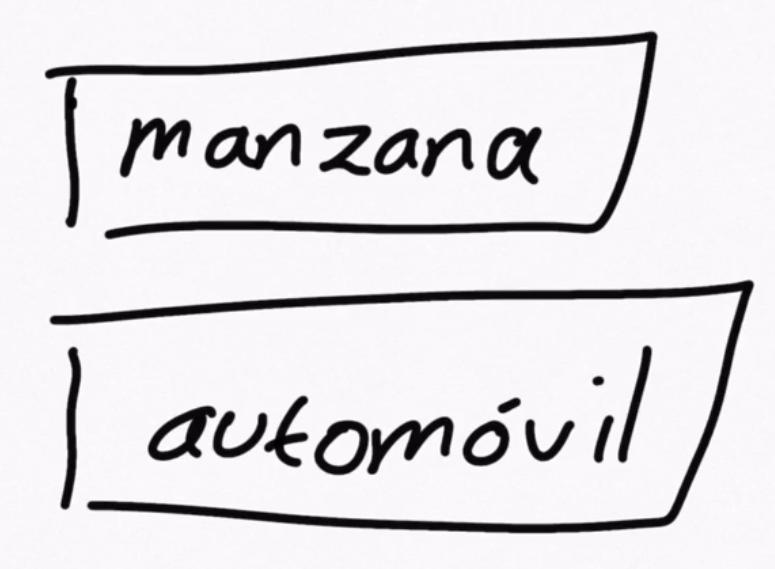
\includegraphics[scale=0.5]{./Pictures/001_entidades.png}
\end{figure}

\newpage
Veamos unos diagramas de ejemplo:
\begin{figure}[h!]
    \centering
      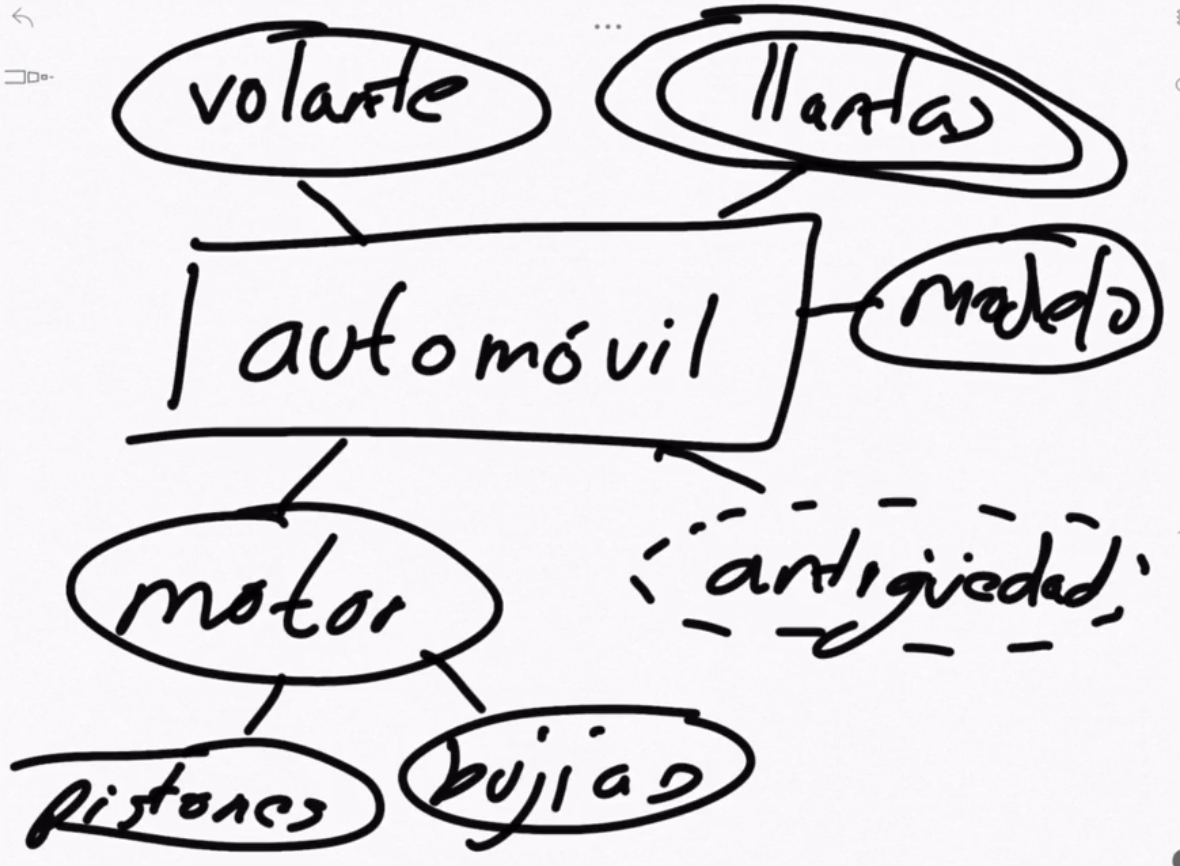
\includegraphics[scale=0.5]{./Pictures/002_Diagrama.png}
\end{figure}

El atributo llantas es un atributo multivaluado, eso quiere decir que la
entidad automóvil tiene más de uno de estos atributos. Como se vé se representa
con un ovalo doble.\\

Ahora veamos el atributo motor es un atributo compuesto ya que, este a su vez
está formado por otros atributos.\\

También fijémonos en el atributo especial llamado antiguedad, ya que este
atributo se puede inferir a partir del año en el que salió el automovil.

\newpage

\begin{figure}[h!]
    \centering
      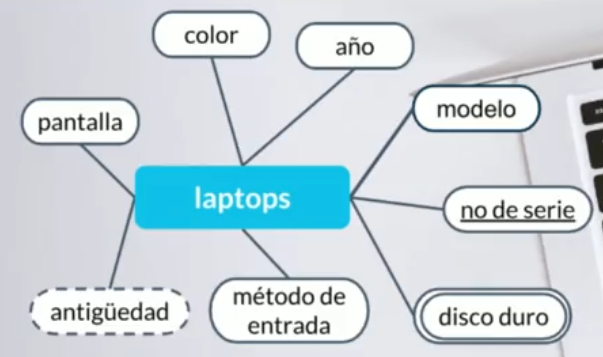
\includegraphics[scale=0.5]{./Pictures/003_atributos.png}
\end{figure}

Por convención las entidades se ponen en plural.\\

En caso del atributo \textbf{no\_de\_serie} es el que diferencia nuestra
entidad de otras y se conoce como atributo llave, se grafica dentro de un óvalo
y además tiene subrayado. Los \textbf{atributos llave} son aquellos que identifican a la entidad y no
pueden ser repetidos.

\begin{figure}[h!]
    \centering
      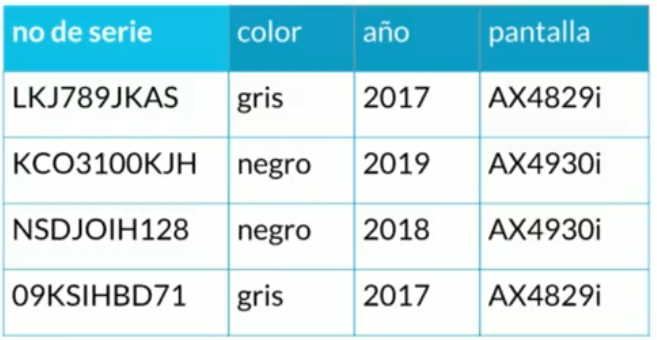
\includegraphics[scale=0.5]{./Pictures/004_id.png}
\end{figure}

Los \textbf{atributos compuestos} son aquellos que tienen atributos ellos
mismos.

Los \textbf{atributos llave} son aquellos que identifican a la entidad y no
pueden ser repetidos. Existen:

\begin{itemize}
  \item Naturales: Son inherentes al objeto como el número de serie.
  \item Clave artificial: No es inherente al objeto y se asigna de manera arbritaria.
\end{itemize}

\textbf{Entidades débiles}: No pueden existir sin una entidad fuerte y se representan
con un cuadrado con doble línea.

\begin{figure}[h!]
    \centering
      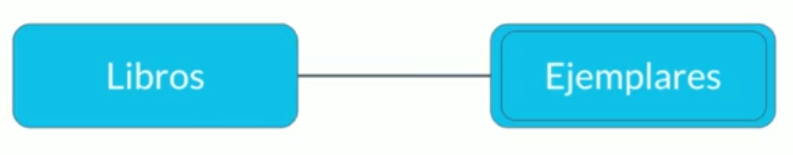
\includegraphics[scale=0.5]{./Pictures/005_entidades_debiles.png}
\end{figure}

Las identidades débiles también se representan con el mismo cuadrado pero
tienen doble línea.

La Identidades pueden ser débiles por dos motivos:\\

\textbf{Entidades débiles por idendidad:} No se diferencian entre si más que
por la clave de su entidad fuerte.

\begin{figure}[h!]
    \centering
      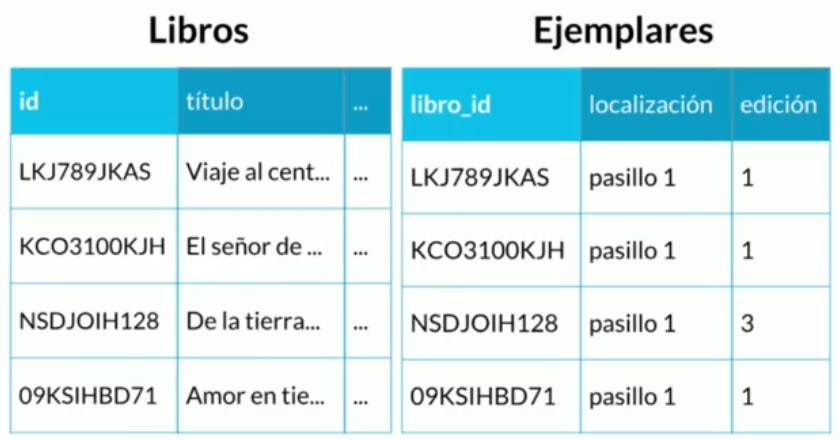
\includegraphics[scale=0.5]{./Pictures/006_entidades_debiles_dependientes.png}
\end{figure}

\textbf{Entidades débiles por existencia}: Se les asigna una clave propia,
pero conceptualmente no puede existir esta identidad sin otra que sea fuerte.

\begin{figure}[h!]
    \centering
      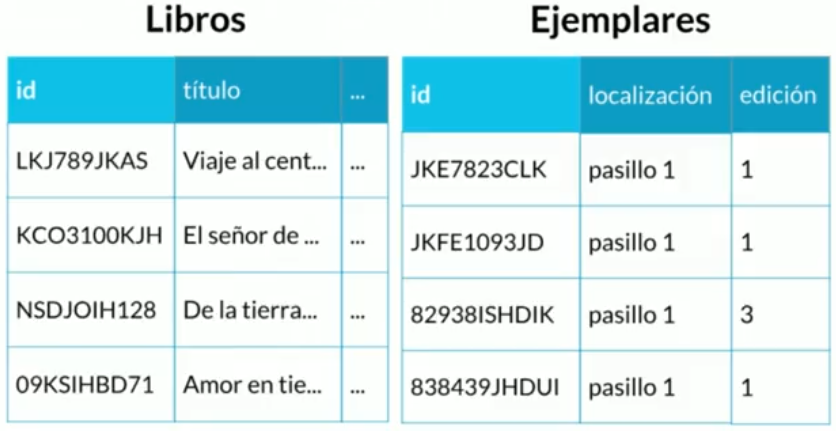
\includegraphics[scale=0.5]{./Pictures/007_enditad_debil_existencia.png}
\end{figure}


%% Clase 4
\section{Entidades de Platzi Blog}%
Nuestro proyecto será un manejador de Blogpost. Es un contexto familiar y nos
representará retos muy interesantes.\\

Primer paso: Identificar las entidades.\\
Segundo paso: Pensar en los atributos.\\

Diagrama ER (Entidad - Relación): Platziblog\\

Veamos las entidades
\begin{figure}[h!]
    \centering
      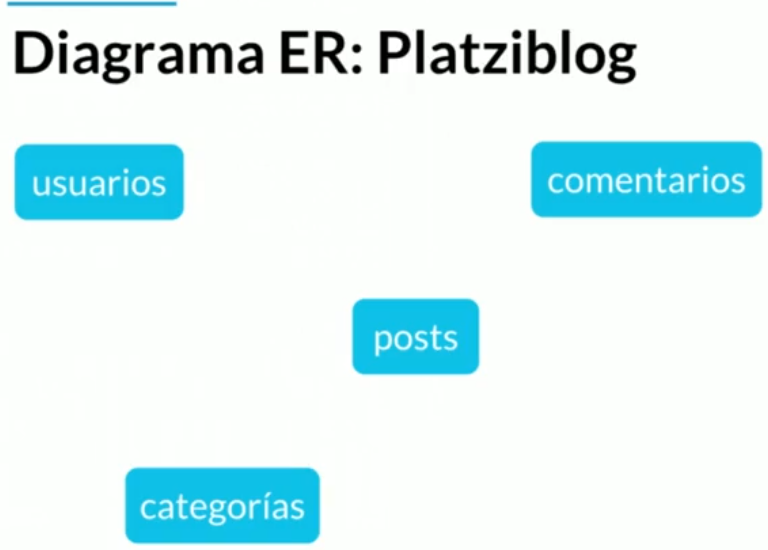
\includegraphics[scale=0.45]{./Pictures/008_Diagrama.png}
\end{figure}

Ahora los atributos de cada Entidad:

\begin{figure}[h!]
    \centering
      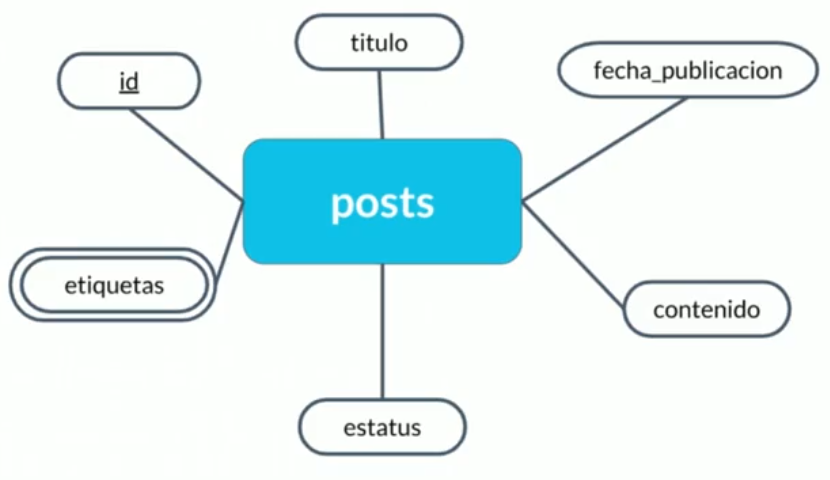
\includegraphics[scale=0.45]{./Pictures/009_post.png}
\end{figure}

\begin{figure}[h!]
    \centering
      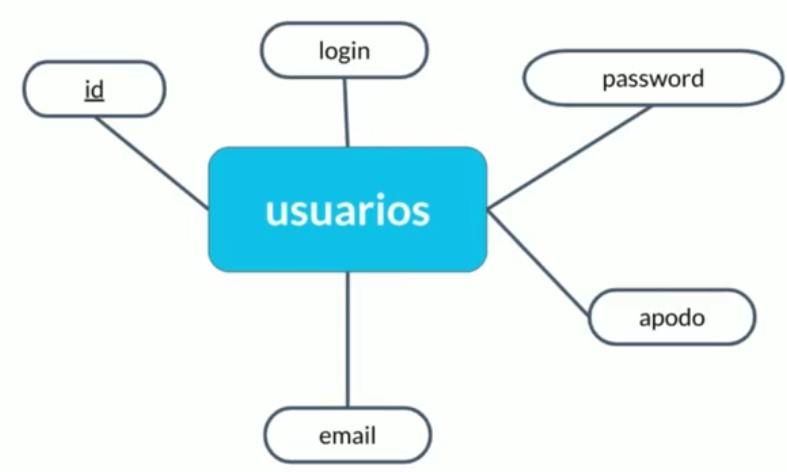
\includegraphics[scale=0.45]{./Pictures/010_usuarios.png}
\end{figure}


%% Clase 5
\section{Relaciones}%
Las \textbf{relaciones} nos permiten ligar o unir nuestras diferentes entidades
y se representan con rombos. Por convención se definen a través de verbos.\\

Por ejemplo veamos dos entidades, \textbf{Automóvil} y \textbf{Dueño} que son
entidades que se van a vincular con la relación lamado \textbf{tiene}.\\

\begin{figure}[h!]
    \centering
      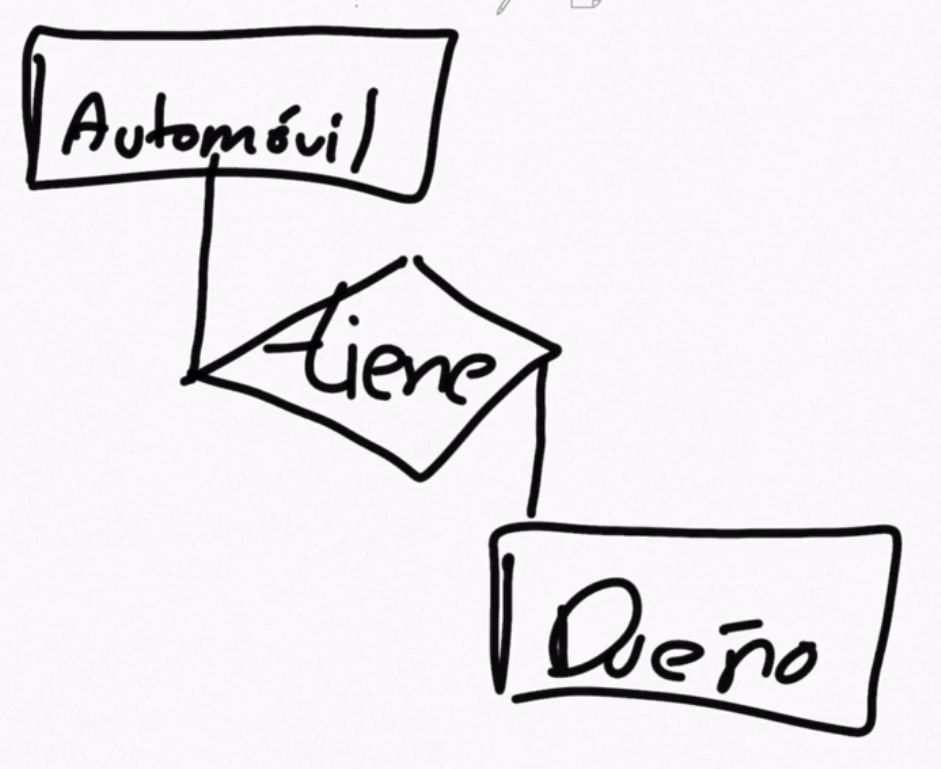
\includegraphics[scale=0.35]{./Pictures/011_relacion_tiene.png}
\end{figure}

Ahora veamos por ejemplo las entidades \textbf{Jugadores} y \textbf{Equipos}
que vamos a vincular con la relación llamado \textbf{pertenece}.

\begin{figure}[h!]
    \centering
      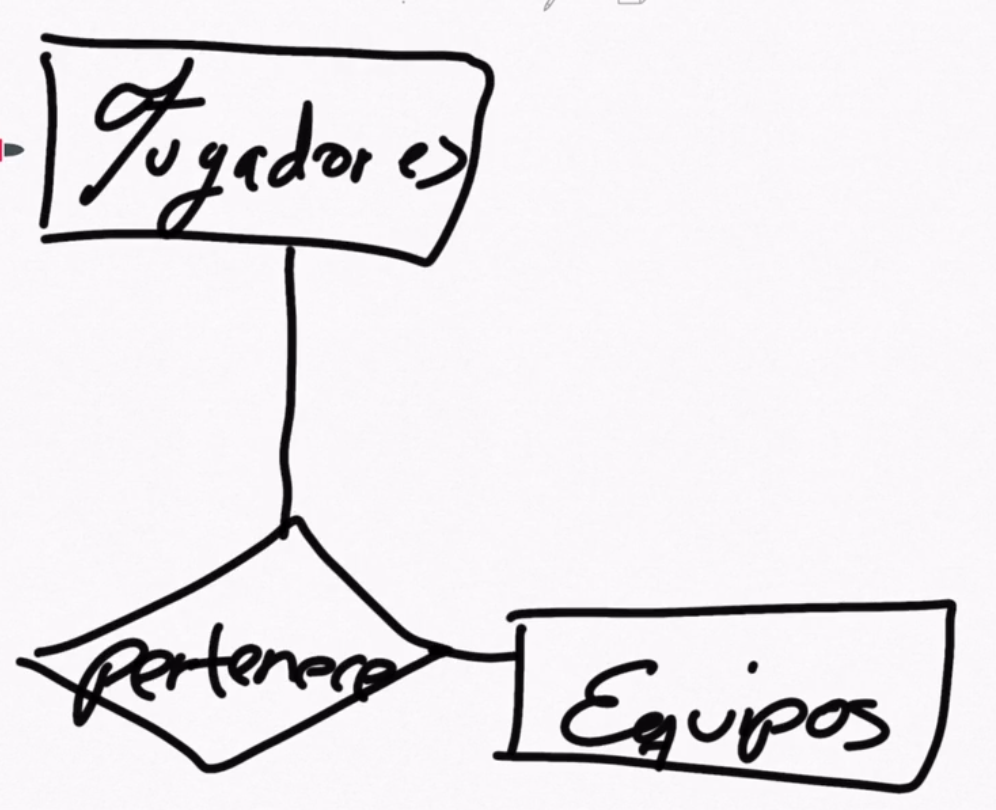
\includegraphics[scale=0.35]{./Pictures/011_relacion_pertenece.png}
\end{figure}

También veamos otras dos entidades: \textbf{laptops} y \textbf{discos\_duros}
(este último era un atributo multivaluado), cuando tenemos atributos
multivaluados por lo general los convertimos en entidades separadas porque
tienen una vida en sí mismas. En este caso decimos que una laptop tiene varios
discos\_duros. Y esto se define con la cardinalidad.

\begin{figure}[h!]
    \centering
      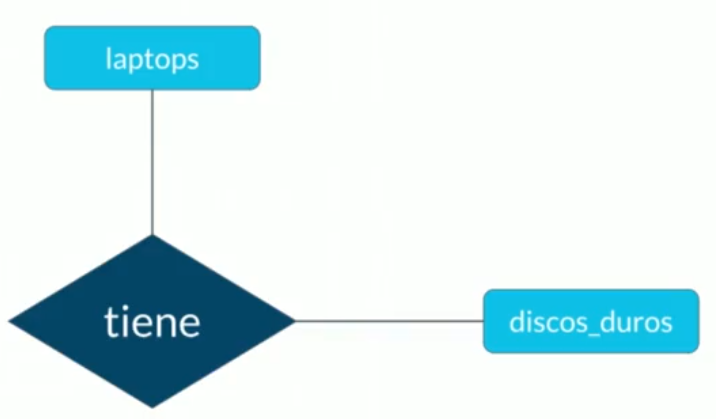
\includegraphics[scale=0.45]{./Pictures/012_relacion_tiene.png}
\end{figure}

En el slide de laptos tiene discos\_duros, se ve que éste ultimo no estaba
siendo considerado una entidad sino que era un atributo multivaluado. Por lo
general a los atributos multivaluados los convertimos en entidades separadas
porque tienen una vida por sí misma y porque se pueden relacionar de diferentes
maneras.\\

Las relaciones tienen una propiedad llamada \textbf{cardinalidad} y tiene que
ver con números. Cuántos de un lado pertenecen a cuántos del otro lado:\\

\begin{itemize}
  \item Cardinalidad: 1 a 1
  \item Cardinalidad: 0 a 1
  \item Cardinalidad: 1 a N
  \item Cardinalidad: 0 a N
\end{itemize}

\textbf{Cardinalidad: 1 a 1}\\
Por ejemplo veamos la cardinalidad de una entidad \textbf{persona} con
\textbf{datos\_contacto}. Vamos hacer el enunciado de 1 \textbf{persona}
cuántos \textbf{datos\_contacto} tiene y esa relación es de 1 a 1. De igual
manera analizamos pero en sentido contrario, 1 \textbf{datos\_contacto}
pertenecen a 1 \textbf{persona}. Para obtener la cardinalidad se verifica el
mayor número de ambos lados. Que en este caso es 1 a 1.

\begin{figure}[h!]
    \centering
      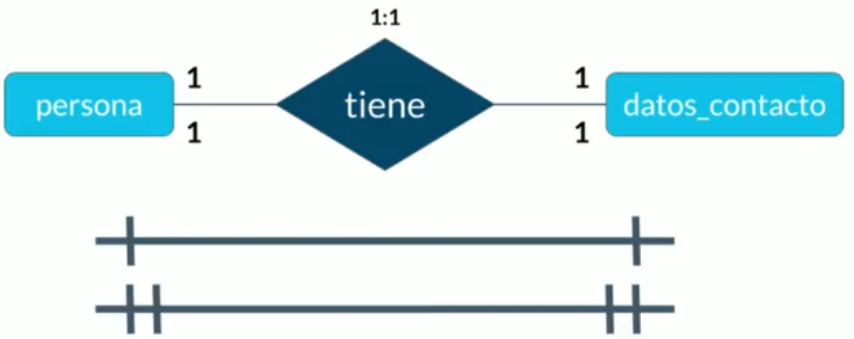
\includegraphics[scale=0.45]{./Pictures/014_card_1_1.png}
\end{figure}

Este diagrama es llamado de \textbf{Entidad Relación}. Esta relación también se
puede representar con el conector que se ve en el grafico, que es llamado
diagrama físico de base de Datos.\\

\textbf{Cardinalidad: 0 a 1}\\
Esta cardinalidad es opcional, por ejemplo puede que haya una
\textbf{sesion\_actual} para un usuario como tambien que no.

\newpage

\begin{figure}[h!]
    \centering
      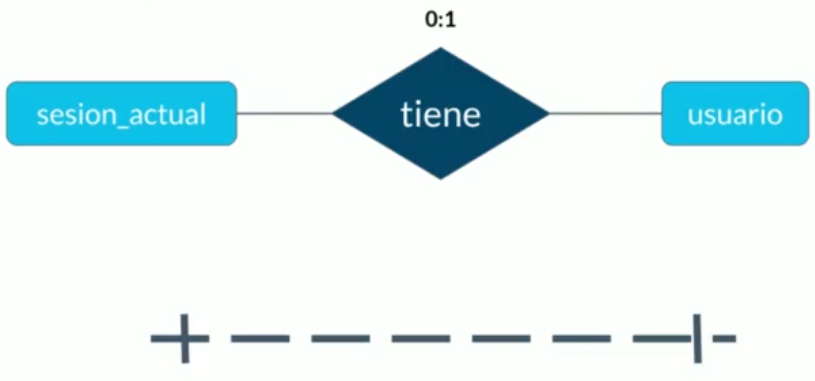
\includegraphics[scale=0.45]{./Pictures/015_card_0_1.png}
\end{figure}

\textbf{Cardinalidad: 1 a N}\\
Esta es la cardinalidad 1 a muchos, por ejemplo: Una persona afortunada, puede
tener muchos automóviles, sin embargo un automóvil por tema de papeles y demás
solo puede pertenecer a una persona. De igual forma, para obtener la
cardinalidad se saca el número mayor de cada lado.\\

\begin{figure}[h!]
    \centering
      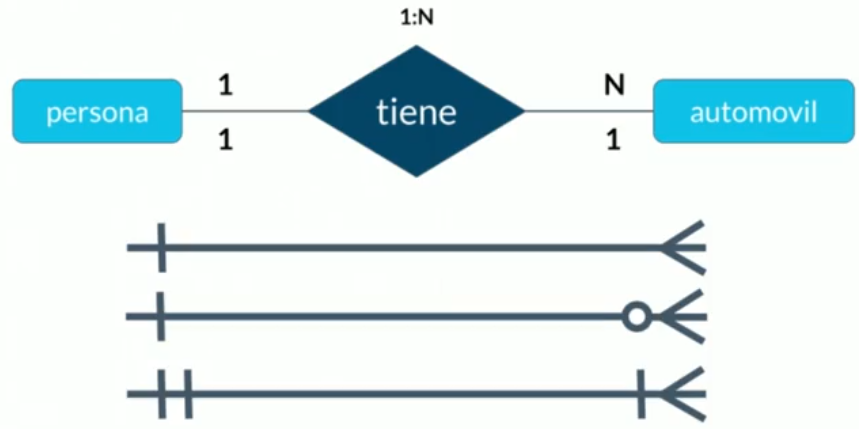
\includegraphics[scale=0.5]{./Pictures/016_card_1_N.png}
\end{figure}

\textbf{Cardinalidad: 0 a N}\\
Por ejemplo en el siguiente esquema podemos observar que una hab\_hospital
puede tener muchos pacientes, pero también puede estar vacía, es decir es
opcional.

\begin{figure}[h!]
    \centering
      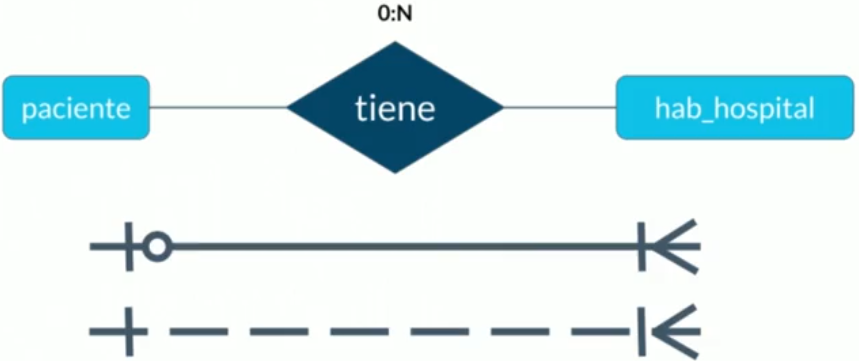
\includegraphics[scale=0.5]{./Pictures/017_card_0_N.png}
\end{figure}


%% Clase 6
\section{Multiples muchos}%
Es un tipo de cardinalidad muy especial. Se verá más adelante cuando se vean
los campos claves y cómo se relacionan las entidades a través de los campos
claves.\\

Esta cardinalidad es de muchos a muchos. Por ejemplo veamos las entidades
\textbf{alumno} y \textbf{clase}. Un alumno puede tomar muchas clases. Una
clase contiene a varios alumnos. En este caso es difícil saber de donde viene
la relación, si es el alumno el que se relaciona con la clase o es la clase la
que tiene muchos alumnos.

\newpage

\begin{figure}[h!]
    \centering
      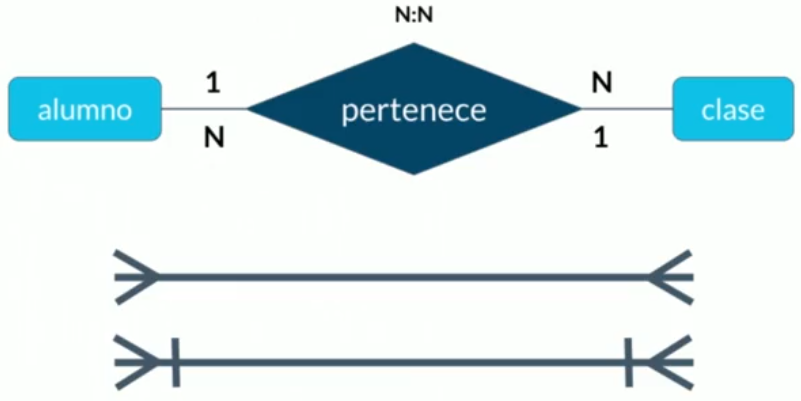
\includegraphics[scale=0.5]{./Pictures/018_card_N_N.png}
\end{figure}


%% Clase 7
\section{Diagrama ER}%
Un diagrama es como un mapa y nos ayuda a entender cuáles son las entidades con
las que vamos a trabajar, cuáles son sus relaciones y qué papel van a jugar en
las aplicaciones de la base de datos.

\begin{figure}[h!]
    \centering
      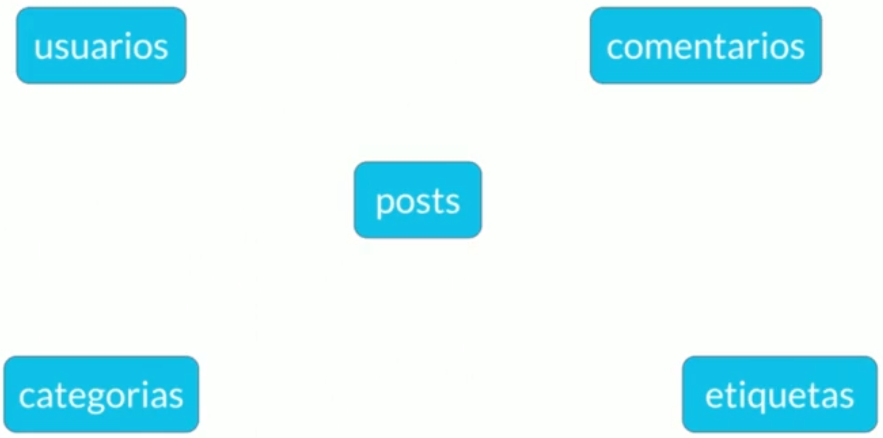
\includegraphics[scale=0.5]{./Pictures/018_DiagramaER.png}
\end{figure}

\begin{figure}[h!]
    \centering
      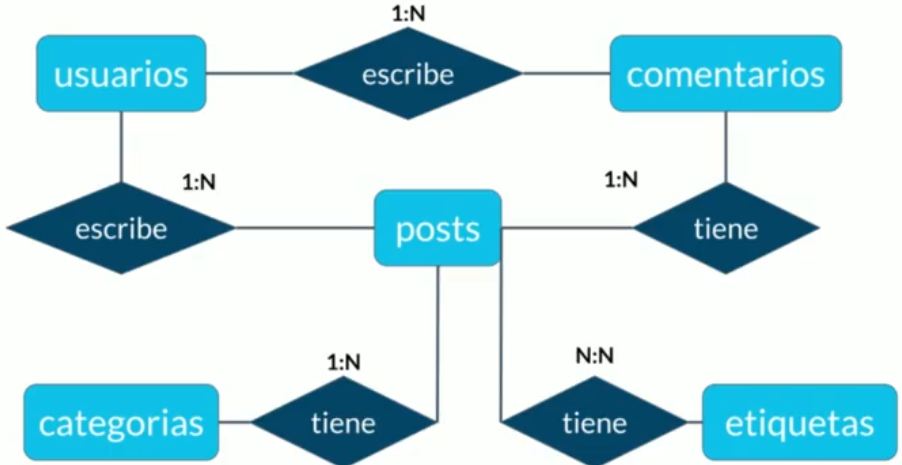
\includegraphics[scale=0.5]{./Pictures/019_diagrama_ER.png}
\end{figure}

%% Clase 8
\section{Diagrama Físico: tipos de datos y constraints}%
Para llevar a la práctica un diagrama debemos ir más alla y darle detalle con
parámetros como:

\textbf{Tipos de datos:}
\begin{itemize}
  \item \textbf{Texto:} CHAR(n), VARCHAR(n), TEXT.
  \item \textbf{Números:} INTEGER, BIGINT, SMALLINT, DECIMAL(n,s), NUMERIC(n,s)
  \item \textbf{Fecha/hora:} DATE, TIME, DATETIME, TIMESTAMP
  \item \textbf{Lógicos:} BOOLEAN
\end{itemize}

\begin{figure}[h!]
    \centering
      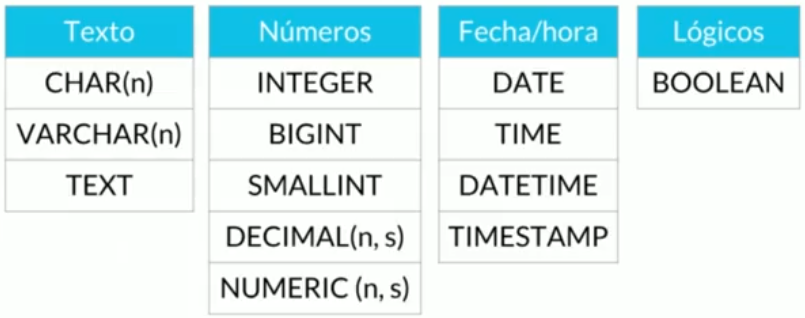
\includegraphics[scale=0.45]{./Pictures/020_tipos_datos.png}
\end{figure}

\textbf{Constraints (Restricciones)}
\begin{itemize}
  \item \textbf{NOT NULL:} Se asegura que la columna no tenga valores nulos
  \item \textbf{UNIQUE:} Se asegura que cada valor en la columna no se repita
  \item \textbf{PRIMARY KEY:} Es una combinación de NOT NULL y UNIQUE
  \item \textbf{FOREIGN KEY:} Identifica de manera única una tupla en otra tabla
  \item \textbf{CHECK:} Se asegura que el valor en la columna cumpla una condición dada
  \item \textbf{DEFAULT:} Coloca un valor por defecto cuando no hay un valor especificado
  \item \textbf{INDEX:} Se crea por columna para permitir búsquedas más rápidas
\end{itemize}

\begin{figure}[h!]
    \centering
      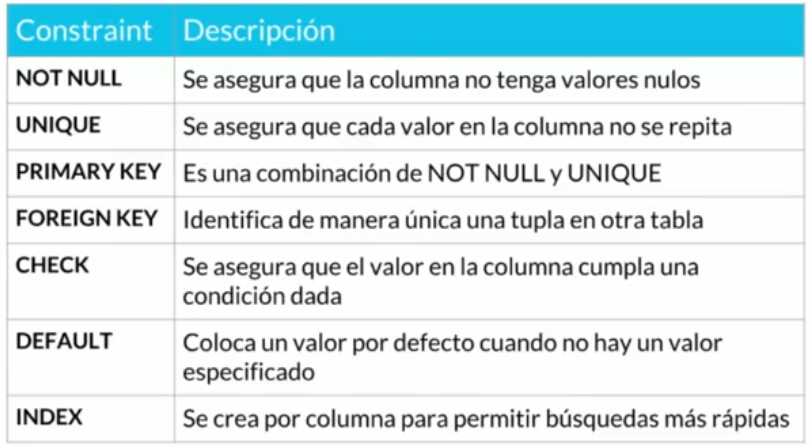
\includegraphics[scale=0.5]{./Pictures/021_constraints.png}
\end{figure}


%% Clase 9
\section{Diagrama Físico: normalización}%
La normalización como su nombre lo indica nos ayuda a dejar todo de una forma
normal. Esto obedece a las 12 reglas de \textbf{Codd} y nos permiten separar
componentes en la base de datos:\\

\begin{itemize}
  \item \textbf{Primera forma normal (1FN):} Atributos atómicos (Sin campos repetidos).
  \item \textbf{Segunda forma normal (2FN):} Cumple 1FN y cada campo de la
    tabla debe depender de una clave única.
  \item \textbf{Tercera forma normal (3FN):} Cumple 1FN y 2FN y los campos que
    NO son clave, NO deben tener dependencias.
  \item \textbf{Cuarta forma normal (4FN):} Cumple 1FN, 2FN, 3FN y los campos
    multivaluado se indentifican por una clave única
\end{itemize}

\newpage
Por ejemplo la siguiente tabla muestra datos \textbf{sin normalizar}:

\begin{figure}[h!]
    \centering
      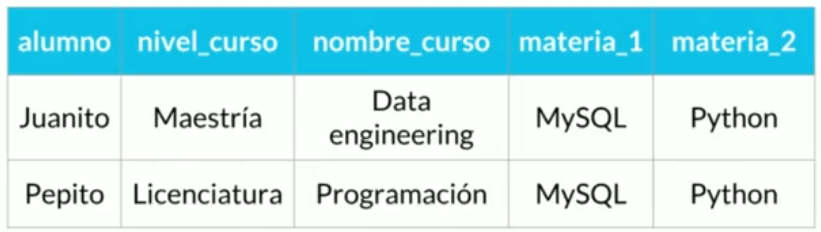
\includegraphics[scale=0.45]{./Pictures/022_sin_normalizar.png}
\end{figure}

Como se verifica en esta tabla, hay campos repetidos materia1 y materia2 que al
fin y al cabo son materia y si se aplica la primera normal entonces tendremos
lo siguiente:

\begin{figure}[h!]
    \centering
      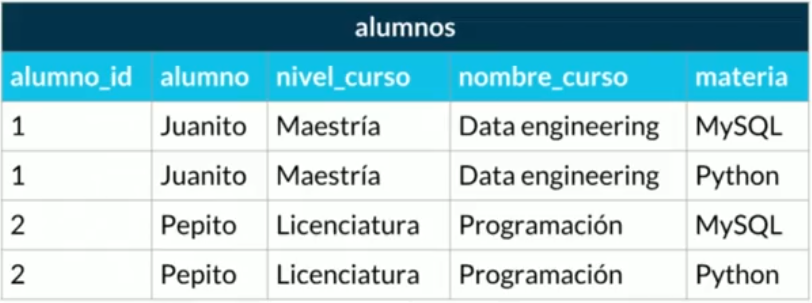
\includegraphics[scale=0.45]{./Pictures/023_primera_normal.png}
\end{figure}

Luego aplicando la segunda regla normal tendremos lo siguiente:
\begin{figure}[h!]
    \centering
      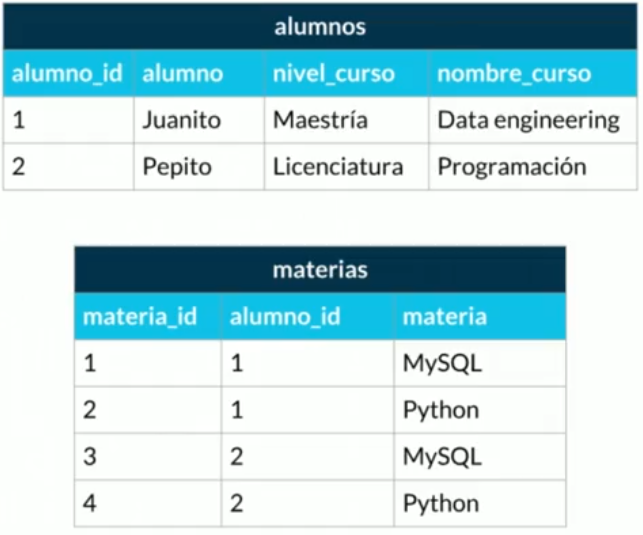
\includegraphics[scale=0.5]{./Pictures/024_segunda_normal.png}
\end{figure}

Ahora a estas tablas aplicaremos la tercera regla normal y obtendremos las siguientes:

\begin{figure}[h!]
    \centering
      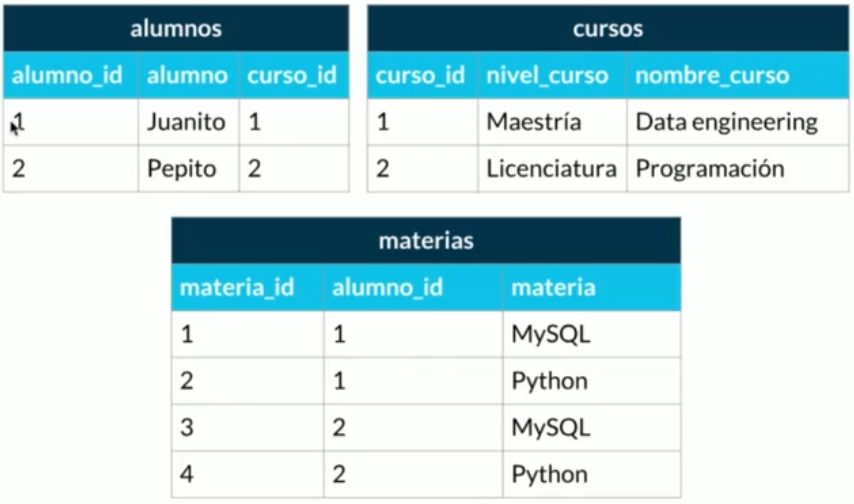
\includegraphics[scale=0.45]{./Pictures/025_tercera_normal.png}
\end{figure}

Finalmente con la cuarta forma normal obtendremos lo siguiente:

\begin{figure}[h!]
    \centering
      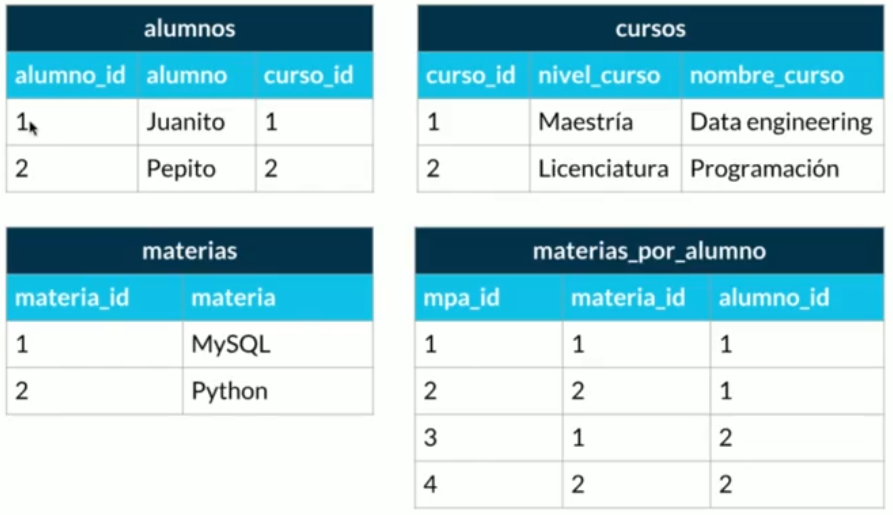
\includegraphics[scale=0.45]{./Pictures/026_cuarta_normal.png}
\end{figure}


%% Clase 10
\section{Diagrama Físico: normalizando Platziblog}%
Comencemos con el diagrama que ya teníamos de Platziblog. Aquí tenemos nuestras
entidades, relaciones y cardinalidad que existe entre ellos.\\

\begin{figure}[h!]
    \centering
      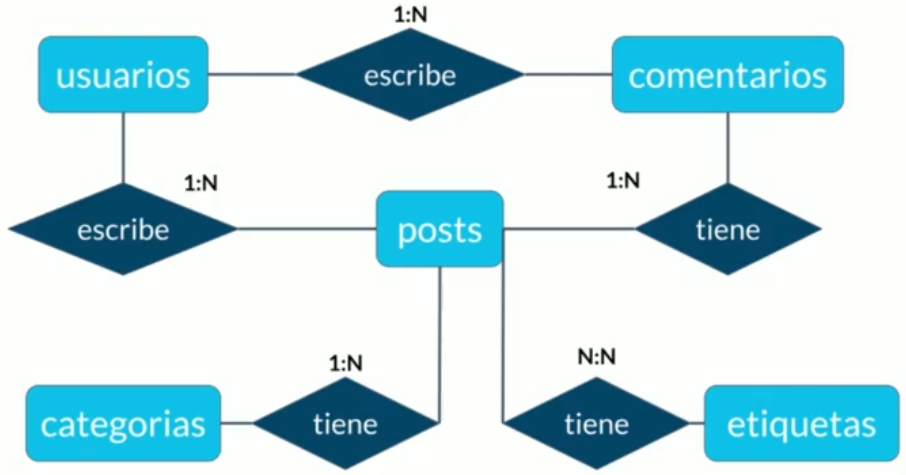
\includegraphics[scale=0.45]{./Pictures/027_diagramaER.png}
\end{figure}

Veamos el diagrama físico:

\begin{figure}[h!]
    \centering
      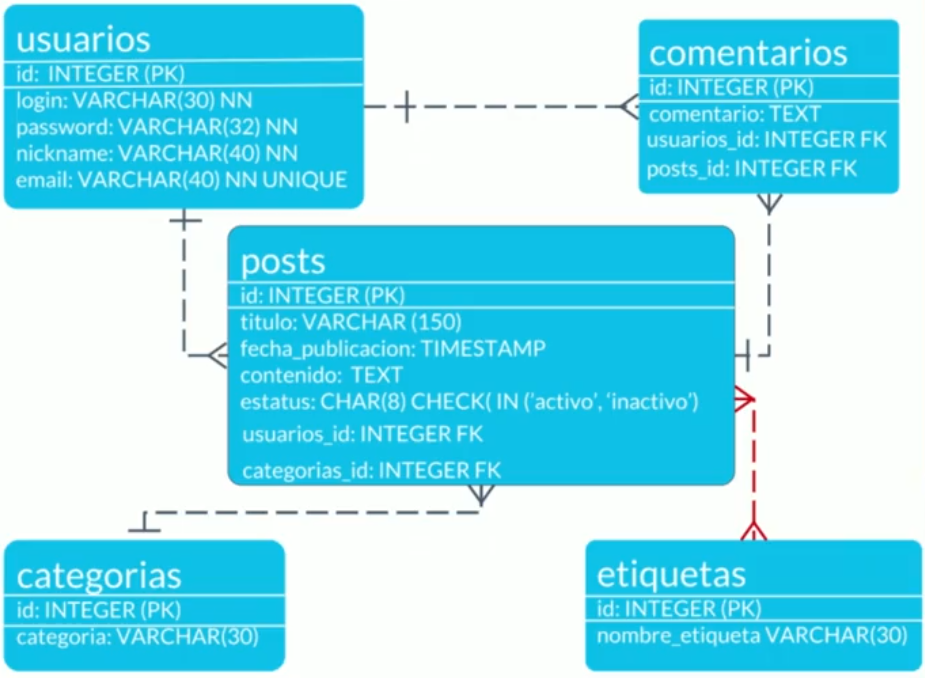
\includegraphics[scale=0.45]{./Pictures/028_diagrama_fisico.png}
\end{figure}

Como se ve en el diagrama en cada relación de 1 a muchos, al que tiene muchos
se le agrega el Foreign Key de la entidad que solo tiene uno en la relación de
cardinalidad. Sin embargo hay que tener en consideración la relación de muchos
a muchos que se verifica entre \textbf{posts} y \textbf{etiquetas}.


%% Clase 11
\section{Formas normales en DB relacionales}%
La normalización en las bases de datos relacionales en uno de esos temas que,
por un lado es sumamente importante y por el otro suena algo esotérico. Vamos a
tratar de entender las formas normales (FN) de una manera simple para que
puedas aplicarlas en tus proyectos profesionales.\\

\textbf{Primera Forma Normal (1FN)}\\
Esta FN nos ayuda a eliminar los valores repetidos y no atómicos dentro de una
base de datos.\\

Formalmente, una tabla está en primera forma normal si:

\begin{itemize}
  \item Todos los atributos son atómicos. Un atributo es atómico si los
    elementos del dominio son simples e indivisibles.
  \item No debe existir variación en el número de columnas.
  \item Los campos no clave deben identificarse por la clave (dependencia
    funcional)
  \item Debe existir una indepencia del orden tanto de las filascomo de las
    columnas; es decir, si los datos cambian de orden no deben cambiar sus
    significados.
\end{itemize}

Se traduce básicamente a que si tenemos campos compuestos como por ejemplo
"nombre\_completo" que en realidad contiene varios datos distintos, en este
caso podrían ser "nombre", "apellido\_paterno", "apellido\_materno", etc.\\

También debemos asegurarnos que las columnas son las mismas para todos los
registros, que no haya registros con columnas de más o de menos.\\

Todos los campos que no se consideran clave deben depender de manera única por
el o los campos que si son clave.\\

Los campos deben ser tales que si reordenamos los registros o reordenamos las
columnas, cada dato no pierda el significado.\\

\textbf{Segunda Forma Normal (2FN)}\\
Esta FN nos ayuda a diferenciar los datos en diversas entidades.\\

Formalmente, una tabla está en segunda forma normal si:
\begin{itemize}
  \item Está en 1FN
  \item Si los atributos no forman parte de ninguna clave dependen de forma
    completa de la clave principal. Es decir, que no existen dependencias
    parciales.
  \item Todos los atributos que no son clave principal deben depender
    únicamente de la clave principal.
\end{itemize}

Lo anterior quiere decir que si tenemos datos que pertenecen a diversas
entidades, cada entidad debe tener un campo clave separado. Por ejemplo.

\begin{figure}[h!]
    \centering
      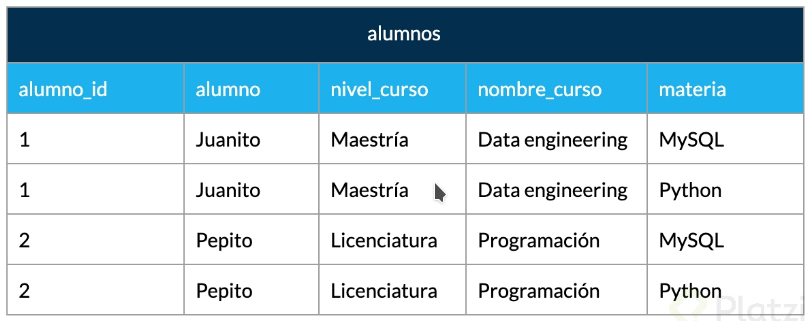
\includegraphics[scale=0.5]{./Pictures/029_normalizacion.png}
\end{figure}

En la tabla anterior tenemos por lo menos dos entidades que debemos separar
para que cada una dependa de manera única de su campo llave o ID. En este caso
las entidades son alumnos por un lado y materias por el otro, ya que una
materia. En el ejemplo anterior, quedaría de la siguiente manera:

\newpage

\begin{figure}[h!]
    \centering
      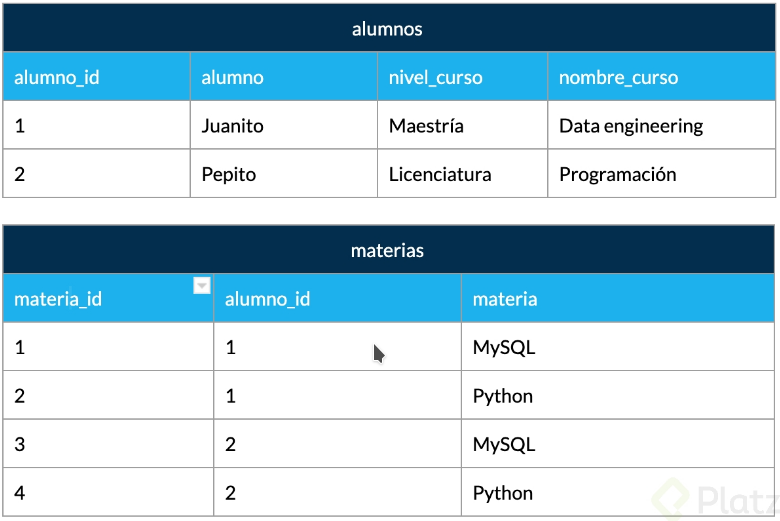
\includegraphics[scale=0.5]{./Pictures/030_normalizacion.png}
\end{figure}

\textbf{Tercera Forma Normal (3FN)}
Esta FN nos ayuda a separar conceptualmente las entidades que no son
dependientes.\\

Formalmente, una tabla está en tercera forma normal si:

Se encuentra en 2FN. No existe ninguna dependencia funcional transitiva en los
atributos que no son clave.

Esta FN se traduce en que aquellos datos que no pertenecen a la entidad deben
tener una independencia de las demás y debe tener un campo clave propio.
Continuando con el ejemplo anterior, al aplicar la 3FN separamos la tabla
alumnos ya que contiene datos de los cursos en ella quedando de la siguiente
manera.

\begin{figure}[h!]
    \centering
      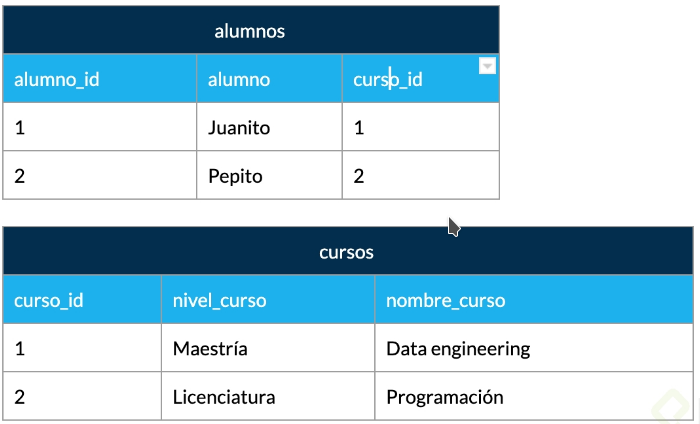
\includegraphics[scale=0.5]{./Pictures/031_normalizacion.png}
\end{figure}

\begin{figure}[h!]
    \centering
      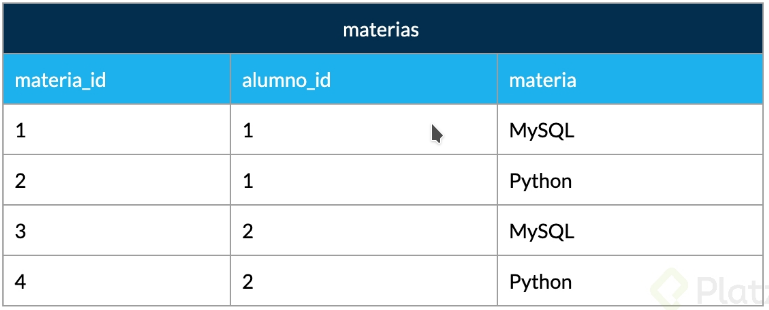
\includegraphics[scale=0.5]{./Pictures/032_normalizacion.png}
\end{figure}

\textbf{Cuarta Forma Normal (4FN)}\\
Esta FN nos trata de atomizar los datos multivaluados de manera que no tengamos
datos repetidos entre rows.\\

Formalmente, una tabla está en cuarta forma normal si:
\begin{itemize}
  \item Se encuentra en 3FN
  \item Los campos multivaluados se indentifican por una clave única
\end{itemize}

Esta FN trata de eliminar registros duplicados en una entidad, es decir que
cada registro tenga un contenido único y de necesitar repetir la data en los
resultados se realiza a través de claves foráneas.\\

Aplicando al ejemplo anterior la tabla materia se independiza y se relaciona
con el alumno a través de una tabla transitiva o pivote, de tal manera que si
cambiamos el nombre de la materia solamente hay que cambiarla una vez y se
propagará a cualquier referencia que haya de ella.

\begin{figure}[h!]
    \centering
      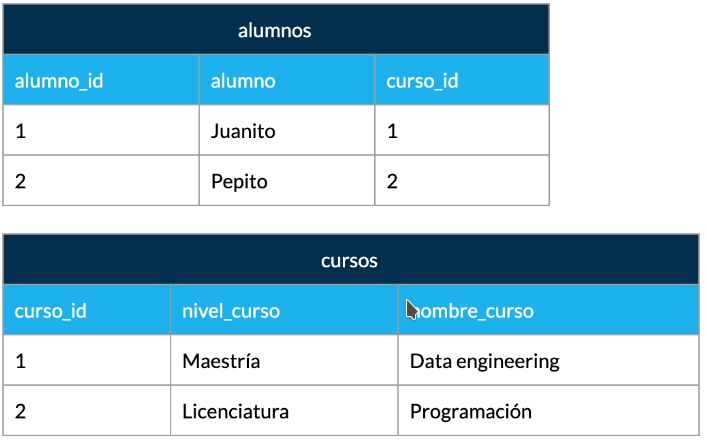
\includegraphics[scale=0.5]{./Pictures/033_normalizacion.png}
\end{figure}

\begin{figure}[h!]
    \centering
      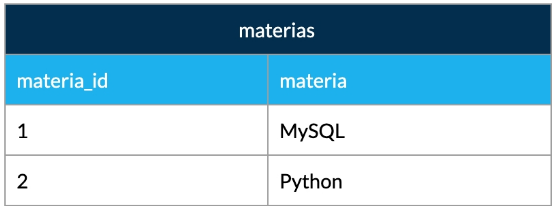
\includegraphics[scale=0.5]{./Pictures/034_normalizacion.png}
\end{figure}

\begin{figure}[h!]
    \centering
      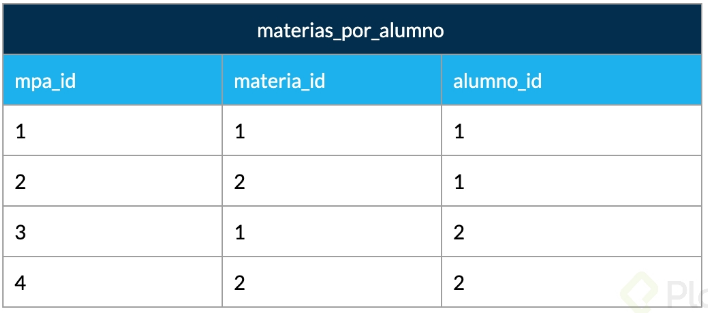
\includegraphics[scale=0.5]{./Pictures/035_normalizacion.png}
\end{figure}

De esta manera, aunque parezca que la infomación se multiplicó, en realidad la
descompusimos o normalizamos de manera que a un sistema le sea fácil de
reconocer y mantener la consistencia de los datos.\\

Algunos autores precisan una 5FN que hace referencia a que después de realizar
esta normalización a través de uniones (JOIN) permita regresar a la data
original de la cual partió.

\newpage

%% Clase 16
\section{Clientes Gráficos}%
\textbf{MySQL Workbench}: Abrimos nuestro cliente gráfico.
\begin{figure}[h!]
  \centering
  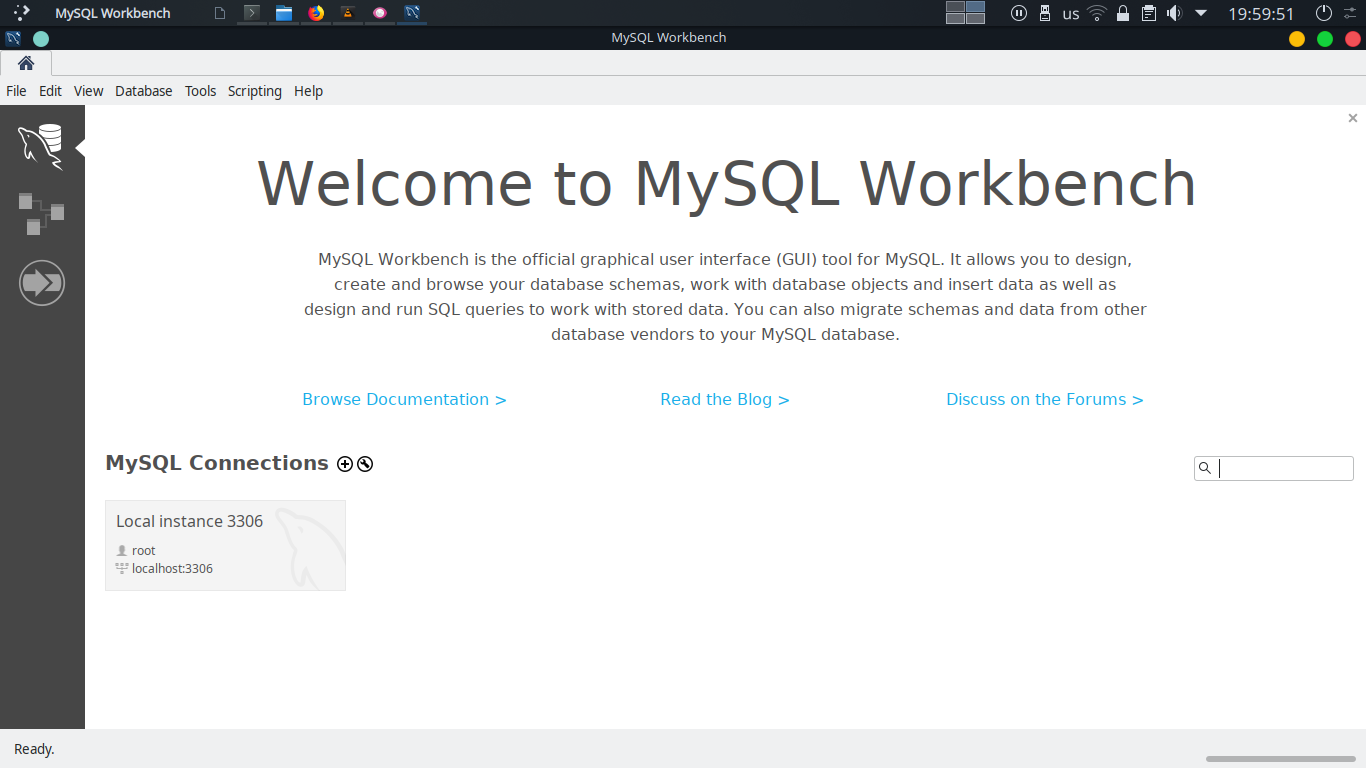
\includegraphics[scale=0.47]{./Pictures/036_workbench.png}
\end{figure}

En la parte inferior nos podemos logear a una conexión, para lo cual nos pedirá
la contraseña para root configurada al momeno de isntalar la base de datos.\\

\begin{figure}[h!]
  \centering
  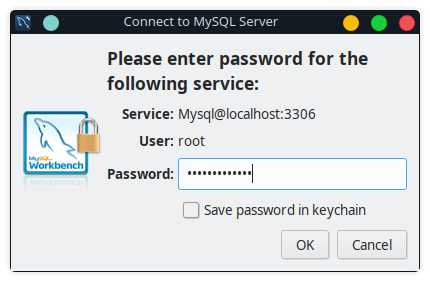
\includegraphics[scale=0.65]{./Pictures/037_local_instance_log.png}
\end{figure}

Veremos como se muestra nuestra área de trabajo y podemos crear un nuevo
esquema de la siguiente manera:

\begin{figure}[h!]
  \centering
  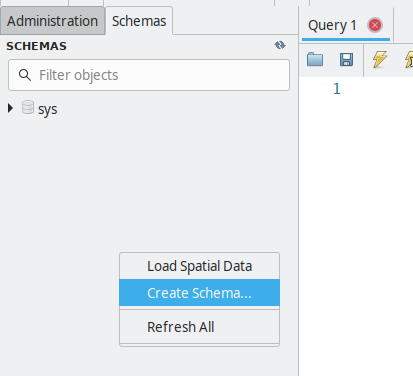
\includegraphics[scale=0.68]{./Pictures/038_create_schema.png}
\end{figure}

\begin{figure}[h!]
  \centering
  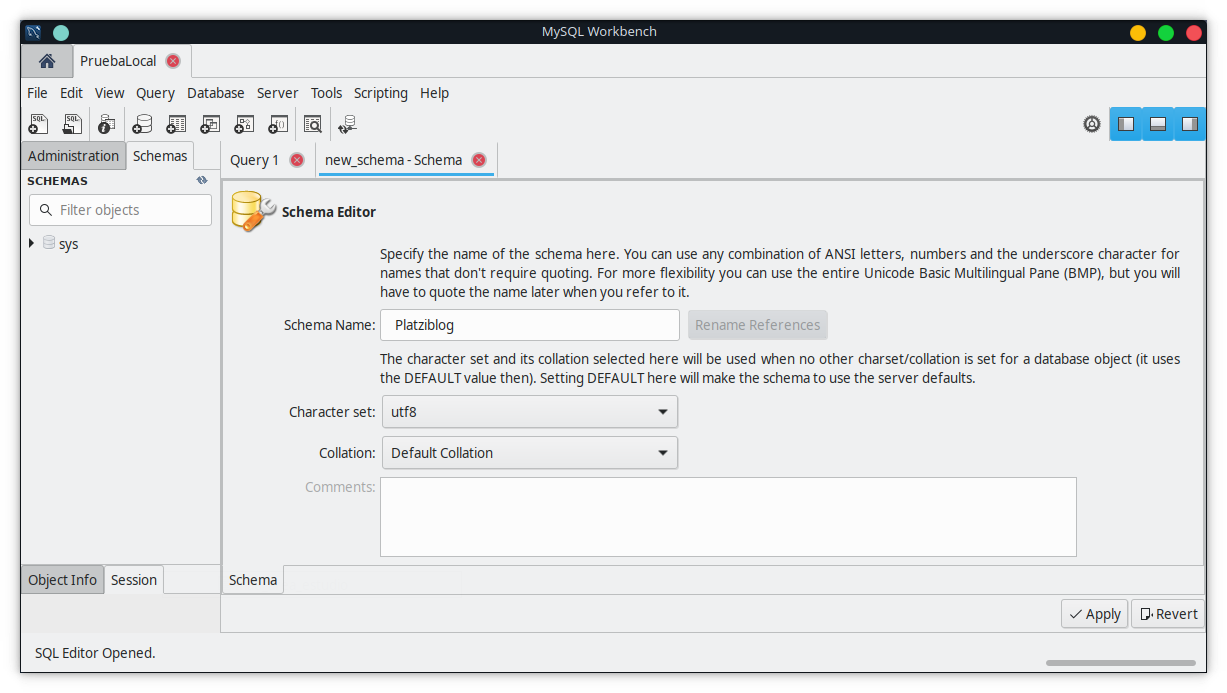
\includegraphics[scale=0.55]{./Pictures/039_create_schema.png}
\end{figure}

\newpage

\begin{figure}[h!]
  \centering
  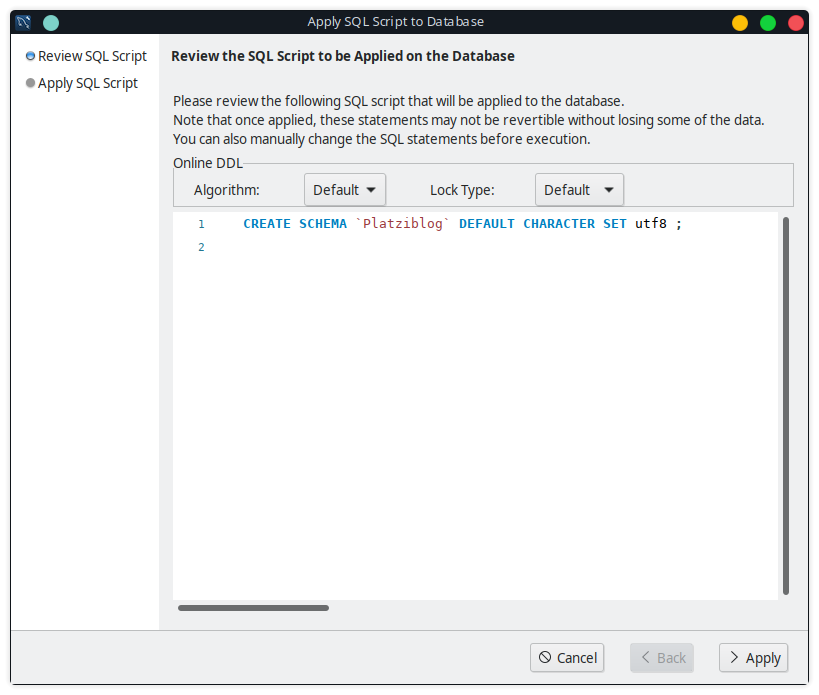
\includegraphics[scale=0.65]{./Pictures/040_create_schema.png}
\end{figure}

\begin{figure}[h!]
  \centering
  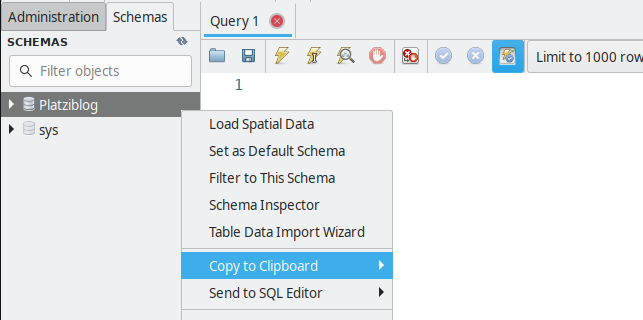
\includegraphics[scale=0.65]{./Pictures/041_create_schema.png}
\end{figure}

\newpage

Luego como vemos en la parte izquierda de nuestra ventana, observaremos el
esquema con el que podremos estar trabajando con diferentes opciones.

\begin{figure}[h!]
  \centering
  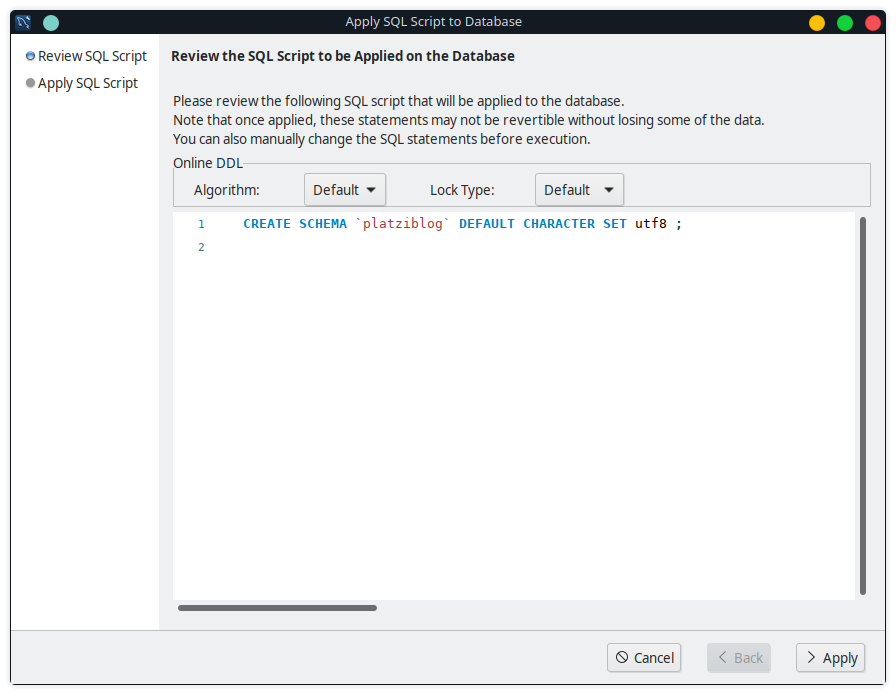
\includegraphics[scale=0.65]{./Pictures/042_create_schema.png}
\end{figure}


%% Clase 17
\section{Servicios administrados}%
Hoy en día muchas empresas ya no tienen instalados en sus servidores los
\textbf{RDBMS} sino que los contratan a otras personas. Estos servicios
administrados cloud te permiten concentrarte en la base de datos y no en su
administración y actualización.\\

Por ejemplo Google Cloud Platform, AWS o Azure te brindan estas posibilidades.

\newpage

%% Clase 18
\section{Historia de SQL}%
\textbf{SQL} significa Structured Query Language y tiene una estructura clara y
fija. Su objetivo es hacer un solo lenguaje para consultar cualquier manejador
de bases de datos volviendose en un gran estándar.\\

Ahora existe el \textbf{NOSQL} o Not Only Structured Query Language que
significa que no sólo se utiliza SQL. Las bases de datos no relacionales.


%% Clase 19
\section{DDL Create}%
\textbf{SQL} tiene dos grandes sublenguajes:\\
\textbf{DDL} o Data Definition Language que nos ayuda a crear la estructura de
una base de datos.\\
Existen 3 grandes comandos:
\begin{itemize}
  \item Create: Nos ayuda a crear bases de datos, tablas, vistas, índices, etc.
  \item Alter: Ayuda a alterar o modificar entidades.
  \item Drop: Nos ayuda a borrar. Hay que tener cuidado al utilizarlo.
\end{itemize}

\textbf{3 objetos que manipularemos con el lenguaje DDL:}
\begin{itemize}
  \item Database o bases de datos
  \item Table o tablas. Son la traducción a SQL de las entidades
  \item View o vistas: Se ofrece la proyección de los datos de la base de datos
    de forma entendible.
\end{itemize}

Vamos a crear un \textbf{schema} llamado Platziblog usando nuestro cliente gráfico.\\
\begin{figure}[h!]
  \centering
  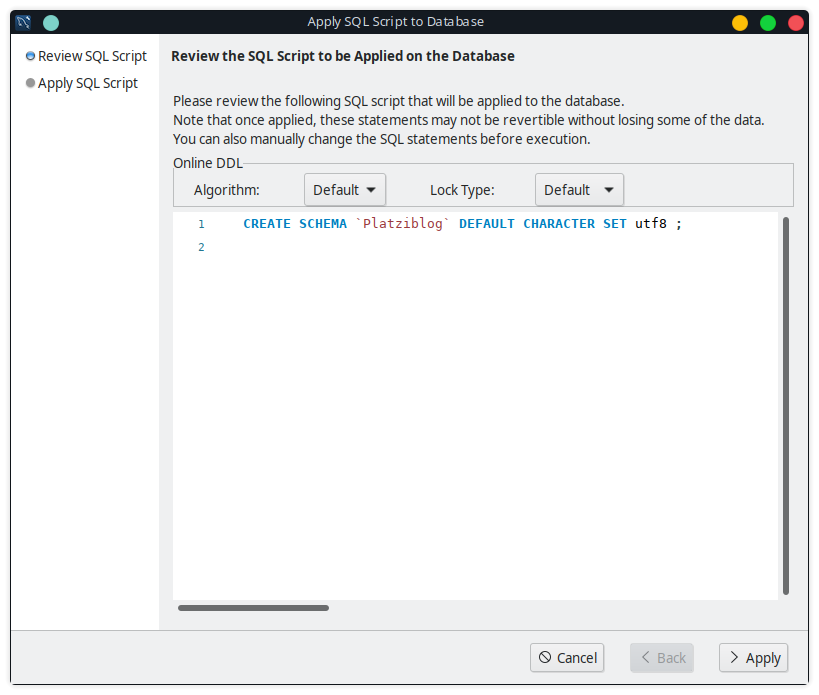
\includegraphics[scale=0.65]{./Pictures/040_create_schema.png}
\end{figure}

Como vemos \textbf{CREATE} es nuestro comando de creación.

\newpage

Ahora vamos a usar nuestro esquema usando nuestro cliente gráfico.\\

\begin{figure}[h!]
  \centering
  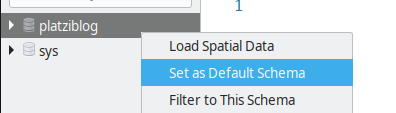
\includegraphics[scale=0.65]{./Pictures/043_use_database.png}
\end{figure}

Esto es equivalente a nuestro comano \textbf{USE DATABASE}\\

Por último vamos a crear una tabla:

\begin{figure}[h!]
  \centering
  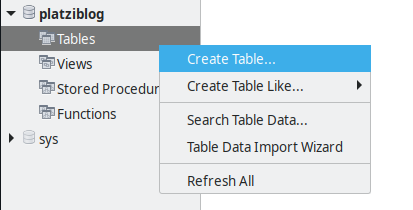
\includegraphics[scale=0.65]{./Pictures/044_create_table.png}
\end{figure}

Agregamos cada uno de nuestros campos.\\

\begin{figure}[h!]
  \centering
  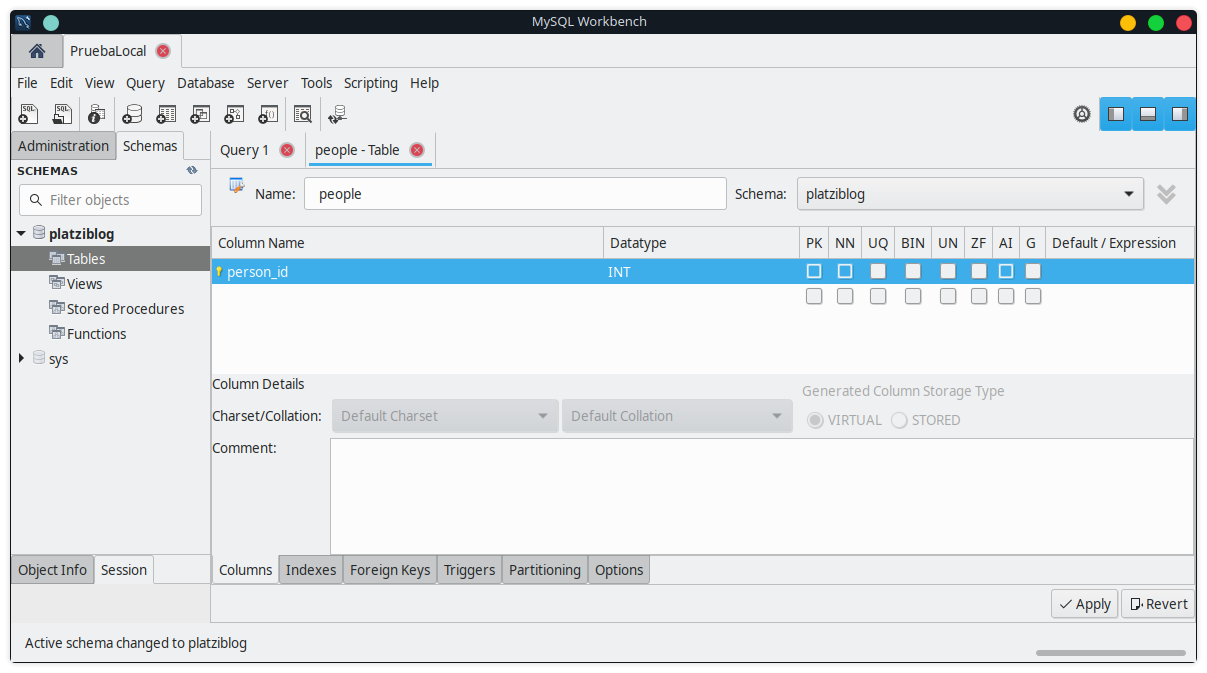
\includegraphics[scale=0.55]{./Pictures/045_person_id.png}
\end{figure}

\newpage
Por defecto nos da marcado el constraint PK (Primary Key) y NN (Not Null).
Podemos agregarle el constraint AI (Auto Increment) para que no tenga el mismo
id nunca.\\

\begin{figure}[h!]
  \centering
  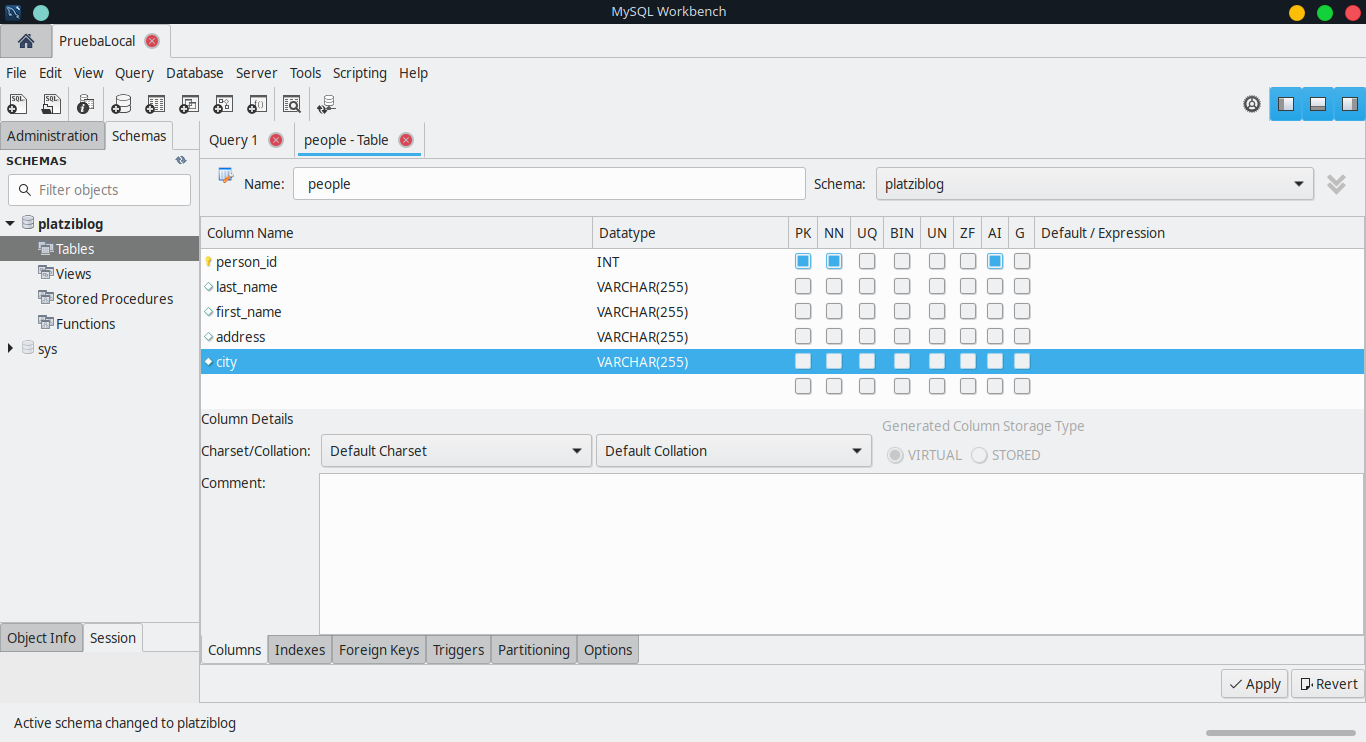
\includegraphics[scale=0.45]{./Pictures/046_people_atributos.png}
\end{figure}

\begin{figure}[h!]
  \centering
  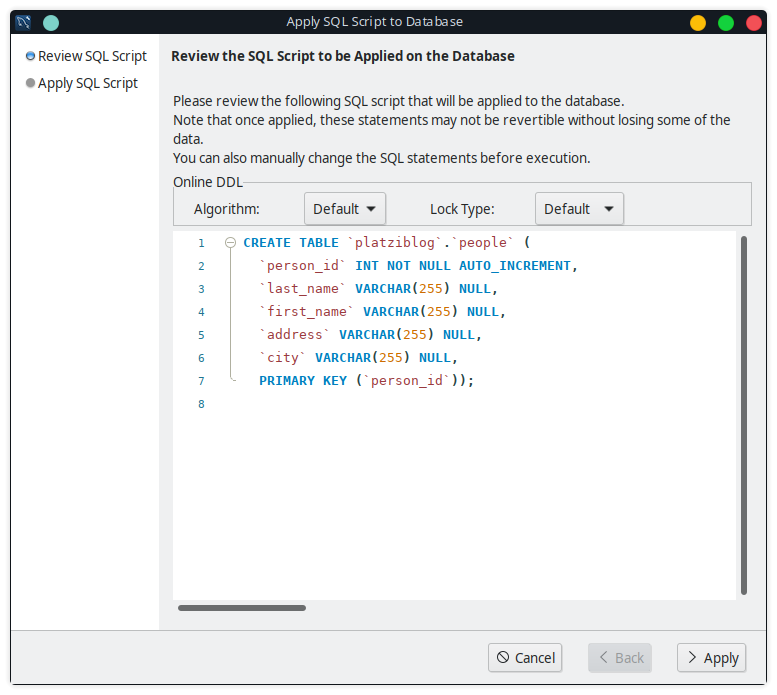
\includegraphics[scale=0.65]{./Pictures/047_people_apply.png}
\end{figure}

Vamos hacer nuestra primera consulta para que veas nuestra tabla quedó bien hecha.\\

\begin{figure}[h!]
  \centering
  \includegraphics[scale=0.75]{./Pictures/048_selec.png}
\end{figure}

\begin{figure}[h!]
  \centering
  \includegraphics[scale=0.75]{./Pictures/049_select.png}
\end{figure}

%% Clase 20
\section{Vistas}%
Vamos a revisar la creación de vistas, tienen que ver con un concepto muy
avanzado y útil. Las vistas lo que hacen es tomar datos de la base de datos,
ponerlos en una forma presentable y convertirlas en algo que podamos consultar
de manera recurrente.\\

\begin{minted}{mysql}
  USE `platziblog`;
  CREATE VIEW `platzi_people` AS
  SELECT * FROM platziblog.people;
\end{minted}

Ahora por ejemplo si seleccionamos con el siguiente comando:

\begin{minted}{mysql}
  SELECT * FROM platziblog.platzi_people;
\end{minted}

Los Views toman datos de la base de datos, los hacen presentables y los
convierten en algo que podamos consultar de manera recurrente.

\section{DDL alter}%
Este comando nos va a permitir modificar nuestra tabla. Por ejemplo agregar una
columna a nuestra tabla o el tipo de un campo, etc.


\vspace{2cm}
\LARGE\textit{RuneCode}


\end{document}

